\documentclass[a4paper,12pt,oneside,openany,titlepage]{jreport}
%\documentclass[a4paper,12pt,oneside,openany]{jsbook} %3/1追加
%\usepackage{graphicx}
\usepackage[dvipdfmx]{graphicx} %1/28追加
\usepackage{fancyhdr}
\usepackage{comment} %1/26追加
\usepackage{amsmath} %1/26追加
\usepackage{indentfirst} %1/29追加
\usepackage{enumitem} % リストの設定調整用
\pagestyle{fancy}
%↓を追加すると,なぜかうまくいく
\renewcommand{\chaptermark}[1]{\markboth{第\ \thechapter\ 章\,\, #1}{}}
\renewcommand{\bibname}{参考文献}
\renewcommand{\baselinestretch}{1.2} %2/8追加

\pagenumbering{arabic}

\begin{document}

% \frontmatter
% \begin{titlepage}
% 表紙 19-39 3/1追加
% begin{titlepage}
%  \vspace*{7mm}
%  \begin{center}
%    \Large{令和4年度 卒業論文}\\
%     \vspace{40truemm}

%    \LARGE{\textbf{TITLE}}\\
%    \vspace{30truemm}

%    \Large{電気通信大学 情報理工学域 I類}\\
%    \Large{メディア報学プログラム}\\

%    \vspace{15truemm}
%    \LARGE{藤山 仁聖} \vspace{5truemm} \\
%    \large{2024 年 3 月} \\
%   \end{center}
% \end{titlepage}

\newpage

% \begin{comment}
\begin{titlepage}
  \vspace*{5mm}
  \begin{center}
    \vspace{-30truemm}
    \LARGE{令和6年度 卒業論文}\\
    \vspace{20truemm}
    {\fontsize{26pt}{0pt} \selectfont \textbf{高難易度アクションゲームに\hspace{10mm}おける人間らしいAI}}


    \vspace{50truemm}
    \Large{電気通信大学 情報理工学域I類}\\
     \Large{メディア情報学プログラム}\\

    \vspace{25truemm}
    \large
      \begin{equation*}
        \begin{split}
          学籍番号&: 2010150\\
          氏名&: 長内勇輝\\
          \vspace{5truemm} \\
          主任指導教員&:清雄一 教授 \\%(直属の人が一番上)
          指導教員&:田原康之 准教授\\
          提出年月日&:2025 年 mm 月 dd日(月) \\
        \end{split}
      \end{equation*}
    \normalsize
    \normalsize

  \end{center}
\end{titlepage}
\newpage
% \end{comment}

\begin{abstract}
  近年,強化学習技術を活用したゲームAIは将棋や囲碁で人間を凌駕しているが, 
  AIの行動は人間に理解しづらく,面白さを損なうことがある.
  生物学的制約や模倣学習を取り入れ,人間らしいプレイスタイルを持つ
  AIの研究が進められているが,複雑な環境となる3Dアクションゲームを
  題材としていることは少ない.
  本研究では,高難易度アクションゲームに対して
  生物学的制約を加えた強化学習を行い,複雑な環境に対応した
  人間らしいゲームAIの提案を行った.
  その後,生物学的制約を加えたAIとそうでないAIのプレイ映像を見せ,
  主観評価を行う被験者実験により人間らしさを評価した.

\end{abstract}

\tableofcontents
\listoftables
\listoffigures
\newpage

%第一章の記述

\chapter{はじめに}
\thispagestyle{fancy}
\lhead{\leftmark}
\rhead{\thepage}
\renewcommand{\headrulewidth}{1pt}

\section{背景}
強化学習技術により,将棋や囲碁などのゲームにおいて人間を凌駕するAIが開発されてきた
.しかし,これらのゲームAIは人間に理解できないような行動や機械的に見える行動をとり,
面白さを損なう場合がある.
そこで近年では,生物学的制約を設けて人間らしいプレイをするゲーム
AIの研究\cite{morita}\cite{tutii}
や,%マリオ,テトリス
模倣学習により人間らしいプレイスタイルをとるゲームAIの研究
\cite{fujiyama}
が行われている.
このような,人間らしいゲームAIは,人間プレイヤを楽しませたり,
難易度調整に利用したりすることが期待されている.

また近年では,プレイヤに難しい操作を求める
高難易度アクションゲームが人気を博している.
高難易度アクションゲームは難易度の調整が重要で,
プレイヤが丁度良く苦戦する難易度にすることが
望ましいとされている.難易度の調整には人間による
テストプレイが必要だが,人間らしいゲームAIがあれば
そのコストを削減することができる.
しかし,高難易度アクションゲームのような3Dアクションゲーム
では,人間らしいAIの研究がほとんどされていないのが現状である.
既存手法では高難易度アクションゲームが持つ複雑な要素に対応できないと
考えられる.
\newpage

\section{高難易度アクションゲーム}
本研究における高難易度アクションゲームとはDARKSOULS\cite{darksouls}
や仁王\cite{niou}のようなゲームを指す.難易度が高いことにより,
プレイヤが何度もゲームオーバーになることから,死にゲーと呼ばれることもある.
基本動作として攻撃,回避,ガードが挙げられ,ゲームの種類によって
様々なアクションが可能となる.

\section{生物学的制約}
生物学的制約とは人間が生きる上で起こりうる身体的
な制約や生き延びようとする心理的な制約のことである.
生物学的制約を加えることによって人間がしない
ような,正確すぎる操作,素早すぎる反応,不自然な
一定の行動をゲームAIがすることを抑制する.
加えてミスをさせることや弱くさせるといった
調整方法をした際に発生しうる「わざとらしさ」
やそれに伴う「つまらなさ」を抑制することができる.

\section{論文の構成}
%TODO:
本論文は第1章から第7章で構成されている.第2章で関連研究,
第3章でオリジナル高難易度アクションゲームについて,
第4章で強化学習の詳細,生物学的制約の検討と導入,
第5章で実験,第6章で考察,第7章で本研究のまとめ,
今後の展望について記す.


\newpage

\chapter{関連研究}
 \thispagestyle{fancy}
 \lhead{\leftmark}
 \rhead{\thepage}
 \renewcommand{\headrulewidth}{1pt}

 \section{DQNと生物学的制約を用いた人間らしい振る舞いのムゲームAI}
 森田はInfinite Mario Bros.で人間らしい振る舞いをするゲームAI
 をDeep Q-Network(DQN)に生物学的制約を加えることで実現させた\cite{morita}.
 生物学的制約として藤井らの先行研究\cite{FuJi_en}
 で使用された「揺らぎ」「遅れ」「疲れ」
 の他,新たに「混乱」「油断」を追加し,「疲れ」をより人間に近くなるように改良した.
 検証として「混乱」と「油断」に対しての実験,改良した「疲れ」に対しての実験
 の2つを行った.それぞれに対して10人の被験者による被験者実験の主観評価
 は提案手法を用いたゲームAIの方が先行研究の手法のみを用いたゲームAI
 よりも,より人間らしい振る舞いをしていると評価された.
 しかし,Infinite Mario Bros.にはスタミナのような
 プレイヤが管理するステータスが存在しなく,
 また,移動,ダッシュ,ジャンプのみの行動で構成されているため,
 ステータスや行動の種類が多い高難易度アクションゲームに
 手法をそのまま適応させることは難しい.
 
 \newpage

 \section{高難易度アクションゲームにおけるプレイヤ
 に気づかれにくい難易度調整手法}\label{teigi}
 荒木らは高難易度アクションゲームにおいて,敵の攻撃状態への遷移確率
 や,攻撃ヒット時のノックバック距離などのプレイヤ
 に気づかれにくい項目を調整することで,プレイヤに察知されること
 なく難易度を調整する方法を提案した.\cite{dif-action}
 
 高難易度アクションゲームの要件を以下のように定めて,
 環境であるゲームを作成した.
 {
\begin{itemize}[itemsep=1pt, leftmargin=27pt, labelsep=5pt, parsep=0pt]
  \item ステータスが高い(HP,攻撃力等)
  \item スーパーアーマーがついた行動をする(攻撃を受けても
  行動が中断されない)
  \item 回復を阻害してくる(回復中に攻撃してくる,
  回復できないように距離を常に詰めてくる)
  \item 盾を構える機会が多い(隙が少ない)
  \item 強力な連続攻撃をする(対処をしないと致命的な攻撃)
  \item 攻撃範囲が広い(敵自体も大きい)
\end{itemize}
}
\newpage



\chapter{オリジナル高難易度アクションゲーム}
 \thispagestyle{fancy}
 \lhead{\leftmark}
 \rhead{\thepage}
 \renewcommand{\headrulewidth}{1pt}


 本研究で扱う環境は,実際に発売されている
 高難易度アクションゲームを参考に,筆者がUnity\cite{unity}で作成した
 3Dアクションゲームである.
 
 \section{ゲームの要件}
 高難易度アクションゲームの要件は\ref{teigi}節のもの
 を参考にし,一部変更を加えた.
 変更点として,常時スーパーアーマー,
 回復を阻害する遠距離からの攻撃,
 ディレイのかかった一撃で瀕死となる攻撃,
 盾を使用しないを加えた.
 
 \section{環境}
 実験環境は図\ref{kankyou}で表す.30*30のフィールドに操作
 可能なPlayerとフローチャートを元に実装したEnemyのみを
 配置し,PlayerかEnemyのHPが0になった時点で1ゲームが終了する.
 Enemyはゲーム開始時,フィールドの4隅からランダムに出現する.
 探索や索敵などには焦点を当てず,戦闘のみの学習を行うため,
 Playerは常時Enemyをロックオンしている状態とした.

 
 \begin{figure}[h]
   \begin{center}
     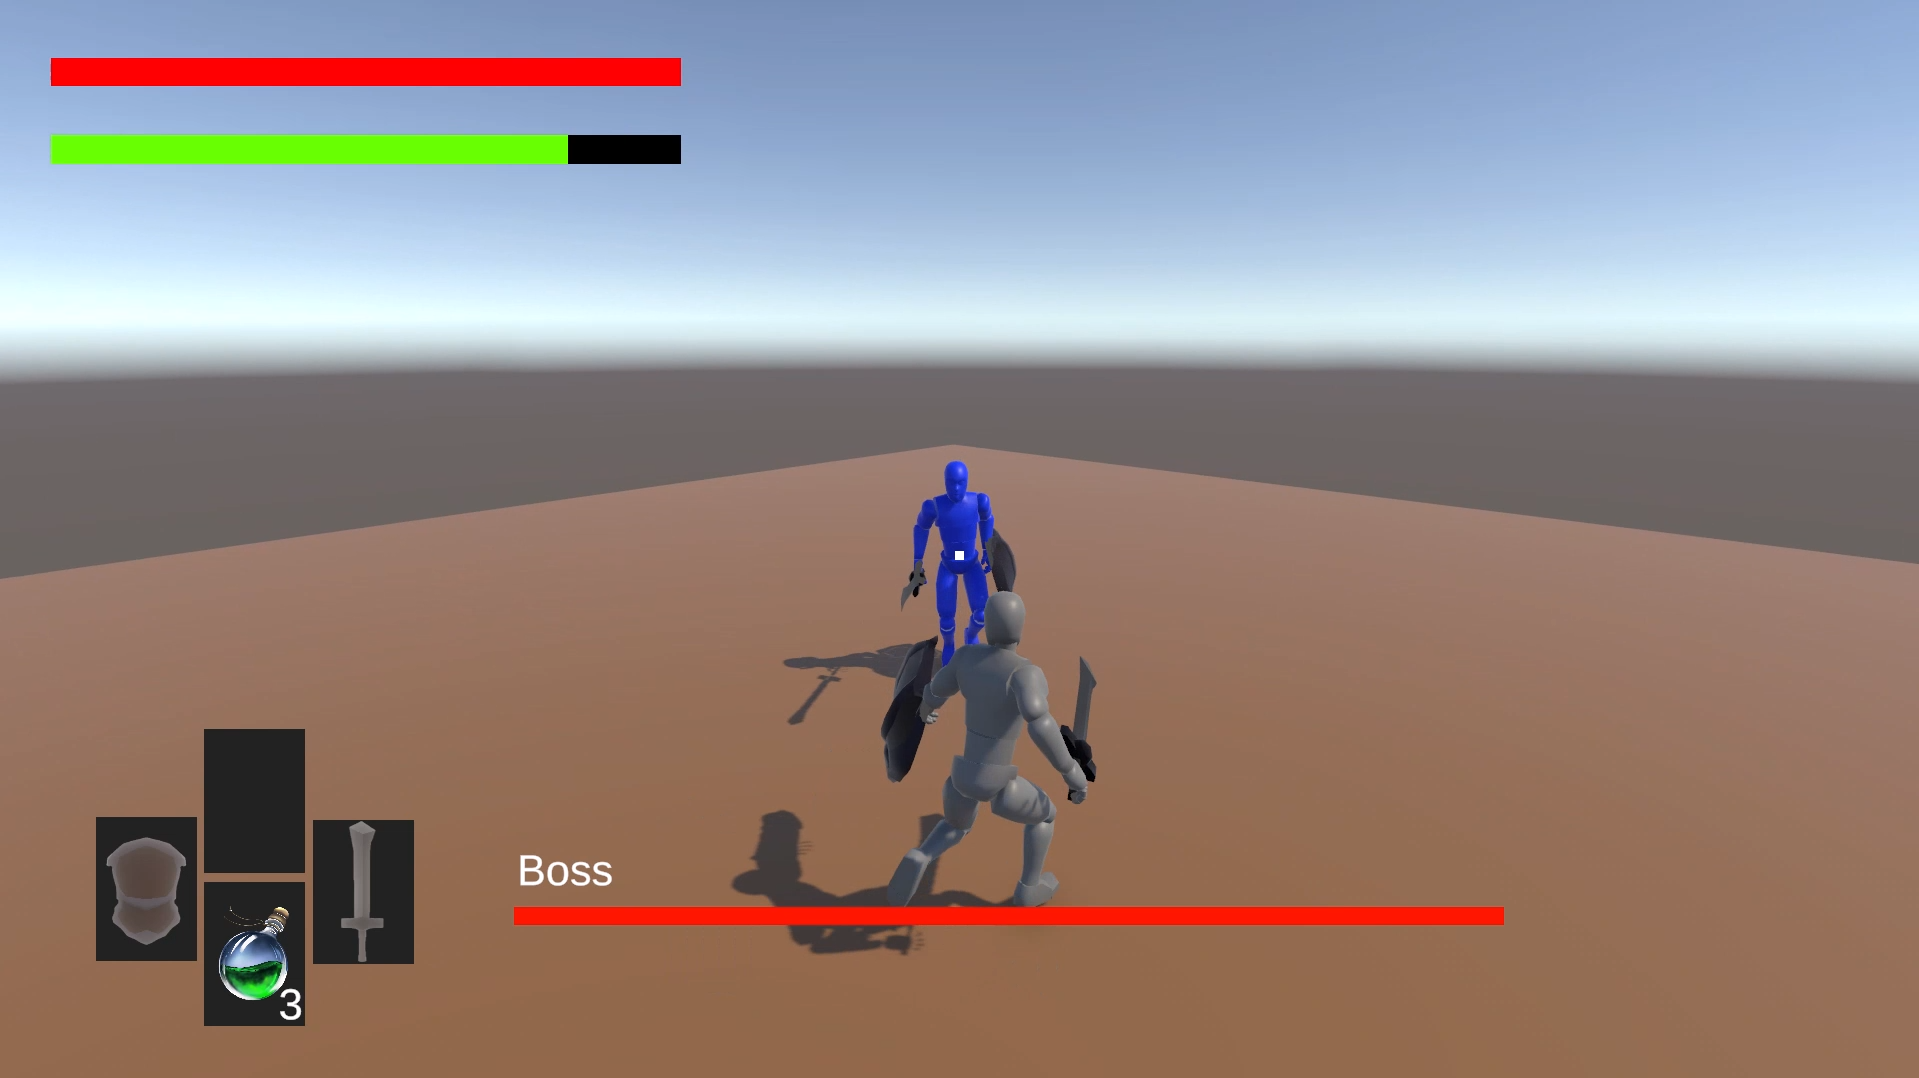
\includegraphics[width=9cm]{ActionGameImage.png}
     \caption{高難易度アクションゲーム環境}
     \label{kankyou}
   \end{center}
 \end{figure}
 
 画面上UIにおいても実際のゲームを参考にし,
 Player,EnemyそれぞれのHPとPlayerのスタミナをバーによって
 表示し,残りの回復数と使用している武器の情報を画面左下に表示した.
 
 \section{アニメーションの作成}
 アニメーションはUnityのPackageである
 Animation Rigging\cite{AnimRigging}を使用して作成した.
 図\ref{anim_controller}のように頭,首,手首,肘,胴体,腰,足
 のボーンと連動して動くコントローラーを設定し,アニメーションを作成した.
 PlayerとEnemyのアニメーションを付録Aに掲載する.
\begin{figure}[h]
  \begin{center}
    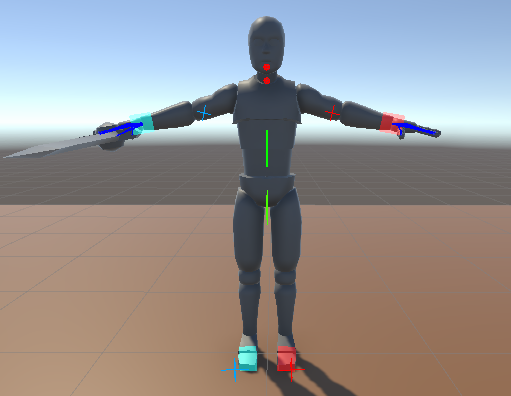
\includegraphics[width=9cm]{Rigging.png}
    \caption{Playerのアニメーションコントローラー}
    \label{anim_controller}
  \end{center}
\end{figure}

 \section{Playerの実装}
 Playerの基本操作は以下の行動を可能とした.
 {
 \begin{itemize}[itemsep=1pt, leftmargin=27pt, labelsep=5pt, parsep=0pt]
   \item Attack1: 右手の剣を使った攻撃
   \item Attack2: 攻撃の直後,連続で入力した際に行う連続攻撃
   \item Guard: 左手の盾を構えてガード
   \item GuardKnockBack: ガード状態で攻撃を受けたときのけぞる
   \item HitKnockBack: ガードしていない状態で攻撃を受けたときのけぞる
   \item GuardBreak: ガード時にスタミナが0の場合,体勢を崩す
   \item Rolling: 転がりながらの回避
   \item RollingAttack: 回避直後に攻撃を入力した際に行う派生攻撃
   \item BackStep: 移動入力がニュートラルの状態で回避を入力
   \item Heal: アイテムを使った回復
   \item Walk: 移動
 \end{itemize}
 }
 それぞれの行動が消費するスタミナと与えるダメージ
 を表\ref{Action_Stamina_Damage}に示す.
Attack1,Attack2,GuardBreak,Heal,Walkは
攻撃を受けたとき,行動が中断されてHitKnockBack状態となる.

HPは100,スタミナは150,回復は3回まで可能とし,
一度の回復で60のHPを回復する.スタミナは通常状態で毎フレーム0.2回復し,
ガード状態では毎フレーム0.1回復する.

 \begin{table}[!ht]
  \centering
  \caption{行動に消費するスタミナと与えるダメージ}
  \label{Action_Stamina_Damage}
  \begin{tabular}{c|c|c}    
  \hline
      行動 & 消費するスタミナ & 与えるダメージ \\ \hline
      Attack1 & 20 & 20 \\ \hline
      Attack2 & 25 & 30 \\ \hline
      Guard & 0 & - \\ \hline
      GuardKnockBack & ガードした攻撃のダメージ値 *1.2 & - \\ \hline
      HitKnockBack & 0 & - \\ \hline
      GuardBreak & 0& - \\ \hline
      Rolling & 20 & - \\ \hline
      RollingAttack & 25 & 15 \\ \hline
      BackStep& 20 & - \\ \hline
      Heal & 0 & - \\ \hline
      Walk& 0 & - \\ \hline
  \end{tabular}
\end{table}


 
 \newpage
 
 \section{Enemyの実装}
 EnemyはHPを500とし,高難易度アクションゲームのボスを
 想定しているためスタミナは使用しない.
 戦闘のみの学習を行うため,Enemyはあらかじめ
 Playerを発見している状態とした.
 Enemyは距離によって行動の選択肢を分け,その中から
 ランダムに選択する.行動の選択肢を図\ref{action_choice}
 に示す.
 
 \begin{figure}[h]
   \begin{center}
     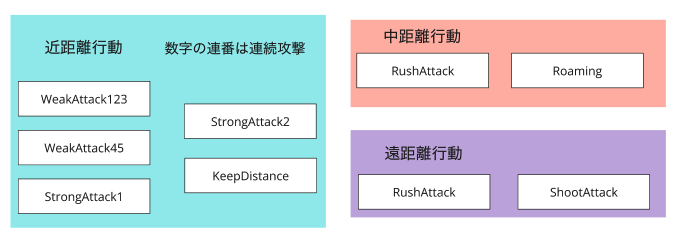
\includegraphics[width=11.5cm]{action_choice_E.png}
     \caption{Enemyの行動選択肢}
     \label{action_choice}
   \end{center}
 \end{figure}
 それぞれの行動の詳細を以下に示す.与えるダメージを括弧内に示す.
 {
  \begin{itemize}[itemsep=1pt, leftmargin=27pt, labelsep=5pt, parsep=0pt]
    \item WeakAttack123: 出が早い3回の連続攻撃.(15,20,30)
    \item WeakAttack45: 2回の連続攻撃,WeakAttack123と比べて攻撃後の隙が長い.(15,30)
    \item StrongAttack1: 単発の刺突攻撃,WeakAttackと比べて攻撃後の隙が長い.(30)
    \item StrongAttack2: 予備動作と攻撃後の隙が最も長く,威力も最も高い攻撃.
          武器の当たり判定に加えて地面にガード不可能の衝撃波を出す.(20,40)
    \item KeepDistance: Playerから距離を取る.
    \item RushAttack: 予備動作の後突進する攻撃.(30)
    \item Roaming: 辺りを彷徨く.
    \item ShootAttack: 空中に浮遊した後,Playerに向かって3回玉を飛ばす攻撃.(20)
  \end{itemize}
  }

 
 Enemyのフローチャートを図\ref{enemy_huro}に示す.Enemy
 はゲームが始まるとPlayerに近づき,近距離行動の範囲
 に入ったとき行動を始める.行動後はPlayer-Enemy間の距離の判定
 を行い,再びランダムに行動をする.以上のことゲーム終了まで繰り返す.
 
 \begin{figure}[h]
   \begin{center}
     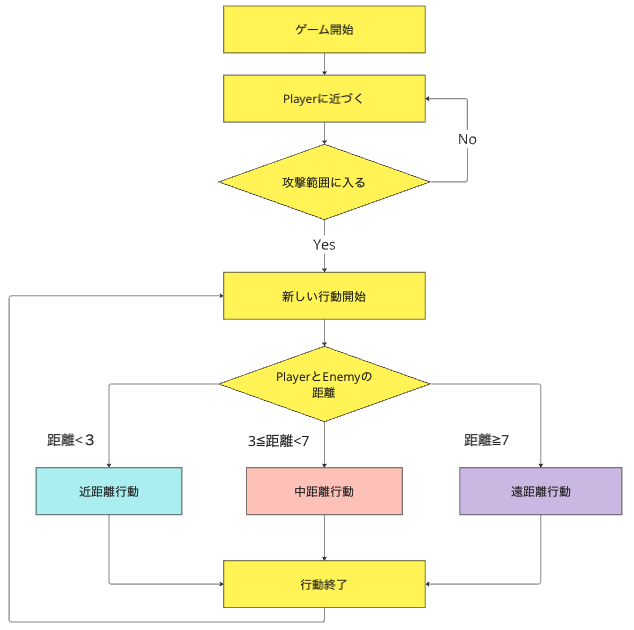
\includegraphics[width=13cm]{enemy_huro.png}
     \caption{Enemyのフローチャート}
     \label{enemy_huro}
   \end{center}
 \end{figure}


\chapter{提案手法}
 \thispagestyle{fancy}
 \lhead{\leftmark}
 \rhead{\thepage}
 \renewcommand{\headrulewidth}{1pt}

 本研究では,作成した高難易度アクションゲームの環境において,
 The Unity Machine Learning Agents Toolkit
 (ML-Agents)の強化学習に生物学的制約を加えることで,
 人間らしさとゲームスキルの高さを兼ね備えたゲームAIの生成
 手法を提案する.
 
 \section{報酬}
 強化学習に用いる報酬は次のように設定した.
 ここでの距離とはPlayerとEnemy間の距離とする.
 %TODO:なぜその報酬を設定したのか説明を入れてもいいかも
 
 \begin{itemize}[itemsep=1pt, leftmargin=27pt, labelsep=5pt, parsep=0pt]
   \item 回復量 * (0.08)
   \item 余剰回復量 * (-0.5)
   \item Playerへのダメージ * (-0.2)
   \item Playerが回避したダメージ * (-0.2)
   \item Enemyへのダメージ * (0.1)
   \item Playerがガードしたダメージ * (0.05)
   \item 攻撃時,距離が4.5以上のとき -4
   \item 攻撃時,距離が1以上2.5以下のとき 0.1
   \item 回復時,距離が3以下のとき -3
   \item 回復時,距離が10以上のとき 0.1
   \item 距離により攻撃を回避をしたとき 0.1
 \end{itemize}
 
 
 \section{観察値}
 観察値は以下のように設定した.
 観察値は人間がプレイしている場合に取得するものと,
 プレイスキルを高めるために必要なものを採用した.
 HP,スタミナ,回復残数,カメラによる画像は,人間が
 プレイしたときに取得する情報である.
 Player,Enemyの座標はPlayer-Enemy間の距離が
 Enemyの攻撃パターンや行動による報酬に関与するため,
 必要であると判断し採用した.
 Enemyの攻撃番号は回避の成功率を高める狙いで採用した.
 
 \begin{itemize}[itemsep=1pt, leftmargin=27pt, labelsep=5pt, parsep=0pt]
   \item Playerの座標 x,y,z
   \item Enemyの座標 x,y,z
   \item PlayerのHP
   \item EnemyのHP
   \item Playerのスタミナ
   \item Playerの回復残数  
   \item Enemyの攻撃番号
   \item Playerに追従するカメラによる画像(256*144)
 \end{itemize}
 
 
 \section{既存の生物学的制約の導入}
 先行研究\cite{morita}にあった生物学的制約のうち「ゆらぎ」「遅れ」「疲れ」「油断」を
 導入する.
 \begin{enumerate}
   \item ゆらぎ(見間違い・操作ミスなど): 人間プレイヤは
   全ての情報を正確に捉えることは不可能であり,また常に正確な操作をすること
   も不可能である.これを再現するためにゲームAIが観測する情報に対してガウスノイズ
   を付与した.ガウスノイズは正規分布に従う乱数をボックス=ミュラー法
   により取得することで実現した.ボックス=ミュラー法は$(0,1]$
   の範囲を取る乱数をX,Y,標準偏差を$\sigma$としたとき,
   (\ref{box_mular_1})(\ref{box_mular_2})
   式で正規分布に従う
   1組の乱数($Z_1,Z_2$)が生成される.
   \vspace{-0.7cm}
   \begin{center}
   \large
   \begin{align}\label{box_mular_1}
   Z_1 = \sigma \sqrt{-2 \log X} cos(2\pi Y)\\
   Z_2 = \sigma \sqrt{-2 \log X} sin(2\pi Y)\label{box_mular_2}
   \end{align}
   \normalsize
   \end{center}
   \vspace{0.3cm}
   $\sigma$の値を0とし,得られた
   ($Z_1,Z_2$)を交互に観察値に加えることで「ゆらぎ」を表現した.   

   \item 遅れ(人間の反射神経): 人間プレイヤは観察した情報
   から実際に操作を行うまでに遅れが発生する.これを再現するために
   アクション決定間隔を数フレーム遅延させた.
   \item 疲れ(キー操作によるもの): 人間プレイヤはコントローラを
   操作することにより疲れが生じ,徐々にパフォーマンスが低下する.
   これを再現するために,疲れの値によって「ゆらぎ」と「遅れ」の
   パラメーターが変化するようにした.
   キー操作の変更ごとに
   $[0,20]$の範囲を取る疲れの値$t$を0.03増加させ,
   $t$の値を0.01倍した値を「遅れ」に加えた.   
   「ゆらぎ」は(\ref{box_mular_1})(\ref{box_mular_2})式
   の$\sigma$に対して$t$を0.05倍した値を加えた.
   よって式は次のようになる.
   \vspace{-0.7cm}
   \begin{center}
   \large
   \begin{align}\label{box_mular_3}
   Z_1 = (\sigma + 0.05t) \sqrt{-2 \log X} cos(2\pi Y)\\
   Z_2 = (\sigma + 0.05t) \sqrt{-2 \log X} sin(2\pi Y)\label{box_mular_4}
   \end{align}
   \normalsize
   \end{center}
   \vspace{0.3cm}

   \item 油断: 人間プレイヤは順調にプレイができているときに
   注意が疎かになり,いつもとは違う行動をとってしまう.これを再現するために
   Playerが10秒間ダメージを受けていない状態でEnemyに攻撃が成功したときから
   次にPlayerがダメージを受けるまでの間を油断状態とし,油断状態では
   ランダム行動の選択確率を$5\%$上昇させた.
   また,ランダム行動時に何もしないダミーの選択肢を混ぜた.
 \end{enumerate}
 
 先行研究では「混乱」をPlayerの周りのオブジェクト数が一定数
 を超えたときに「揺らぎ」と「遅れ」のパラメータを増加することで
 導入していたが,本環境では一対一の戦闘を想定しているため除外した.
 また,高難易度アクションゲームは何度もゲームオーバーになることを想定しているため,
 疲労が蓄積しやすい考えられる.よって「疲れ」の値はゲームが終了しても
 引き継ぐようにし,学習の1エピソードの区切りである
 10ゲーム終了時点でリセットされるようにした.
 これにより,疲れが蓄積される過程を学習させることができるのではないかと考えた.
 
 
 \section{新しい生物学的制約の検討}
 既存の生物学的制約のみでは複雑な環境である
 高難易度アクションゲームに対応することは難しい.
 既存手法に加えて検討する「緊張」「節約」「リスク回避」は
 以下のような理由で採用する.
 
 \begin{enumerate}
  \item 緊張: 緊張はストレス反応の一種であり,人間は
        ストレスや
        プレッシャーがかかると前頭前野の機能が低下し,
        普段しない行動をしてしまうことやミスが増加することがある.
        スポーツの分野ではクライマックスシーンで
        非合理的な行動をすることやプレイの精度が低下することがある.
        長谷川らの研究により,ゴルフプレイヤはプレッシャー下において
        パフォーマンスが低下することが確認された\cite{stress}.
        高難易度アクションゲームも同様に勝敗が決定するような場面では,
        パフォーマンスが低下し,普段しない
        行動をとってしまうと考えられるため採用した.


        %スポーツ心理学の分野では競技のクライマックスシーン
        %での非合理な行動 TODO:ここら辺の論文探したい
  \item 節約: 人間の行動における心理的バイアス
        の一つに保有効果(Endowment effect)があり,所有している
        ものに対して,そのものの性質だけでなく,所有する
        ことによって得られる精神的な報酬にも価値を見出すというものである.
        大橋の研究により,シャープペンシルやマグカップの取引において保有効果
        が示された\cite{hoyuu}.
        この現象はゲームにおいても有効であり,貴重なアイテム
        を使わず,最後まで温存するラストエリクサー症候群
        と呼ばれるものがある.
        よって高難易度アクションゲームにおいても
        回復薬などのアイテムやスタミナなどの
        後に必要となるかもしれないものを温存する行動が
        人間らしさに繋がると考え採用した.


  \item リスク回避: 
        人間は危険が迫ると扁桃体が活性化され,
        回避行動が促進されると言われている.また,
        危機的状況に陥ると,損失回避バイアスが
        働き,利益を得る行動
        よりも損失を避ける行動が優先される.
        よって高難易度アクションゲームにおいても
        ダメージを受け瀕死状態にいるときに危険
        を回避する行動が人間らしさに繋がると考え採用した.
        
\end{enumerate}
先行研究\cite{morita}
のゲームと高難易度アクションゲームには相違点があり,それは
HPやスタミナなどのステータス,攻撃,防御,回避などの
行動から生まれる戦闘の駆け引きである.
「緊張」「リスク回避」は戦闘の駆け引きから生じる人間の心情の変化
を表すことができ,「節約」はステータスやアイテムの使い方
に制約をかけることで,
人間らしくすることができると考えた.
よって,以上の3つの生物学的制約を加えることで,
高難易度アクションゲームに対応した人間らしいAIが生成できると考えた.


\section{新しい生物学的制約の導入}
 「緊張」「節約」「リスク回避」は次のように導入した.
 \begin{enumerate}
   \item 緊張: PlayerかEnemyのHPが30以下のときに緊張状態とし,
   Playerが緊張状態のとき,ランダム行動選択確率を5$\%$増加させた.
         
   \item 節約: Playerのスタミナが20以下のときに-0.05,
   Playerのスタミナが20より大きく40以下のときに-0.03,
   Playerのスタミナが70以上100以下のときに0.02の報酬をそれぞれ与えた.
   加えて回復薬を使用時,最後の一つだった場合に-1の報酬を与えた.        
         
   \item リスク回避: PlayerのHPかスタミナが30以下のときに,
   Player-Enemy間の距離が3以下だった場合-0.02の報酬を与えた.
 
 \end{enumerate}
 


\chapter{実験}
 \thispagestyle{fancy}
 \lhead{\leftmark}
 \rhead{\thepage}
 \renewcommand{\headrulewidth}{1pt}

 本実験では,ゲームAIに生物学的制約を含まないもの,
 含むもの(「ゆらぎ」「遅れ」「疲れ」「油断」),新しい
 生物学的制約の内1つを含むもの(「緊張」「節約」「リスク回避」),
 新しい生物学的制約の内2つを組み合わせたもの,
 新しい生物学的制約を全て含むもの
 をML-Agentsで学習させ,被験者実験によって人間らしさを評価する.
 実験の被験者として高難易度アクションゲームを10時間以上プレイ
 したことがある4人とプレイしたことがない6人の合計10人を集めた.
 
 
 実験で用いられるプレイ映像を表\ref{eizo}に示す.
 生物学的制約を組み合わせた9つのゲームAIと人間によるプレイ映像を用いる.
 それぞれのプレイ映像は「疲れ」の影響がわかりやすくするため,
 10ゲームの後半1分程度をトリミングした.
 
 このプレイ映像では高難易度アクションゲームの攻略
 において有効とされる戦略\cite{fam_kouryaku}の内,
 作成した高難易度アクションゲームに適応できる次のことを意識した.
 \begin{enumerate}
   \item スタミナの管理をしてスタミナをできるだけ枯渇しないようにすること
   \item 攻撃よりも防御を優先すること
   \item 間合いの管理をして敵の攻撃を誘うこと
   \item 敵の攻撃をガードもしくは回避して,その隙に攻撃をすること
 \end{enumerate}
 
 次に被験者にあらかじめ録画された9つのゲームAIまたは人間のプレイ映像
 を見てもらい,7段階で2つの質問「このゲームAIは人間らしい動きをしているか」
 (1が最も機械的な動きを,7が最も人間らしい動きをしているとする),
 「このゲームAIはどのくらいのゲームスキルを持っているか」
 (1が初心者,7が上級者とする)に答えてもらう.
 加えてそれぞれの映像に対して自由記述欄を設けた.
 
 \begin{table}[!ht]
   \centering
   \caption{実験で用いられるプレイ映像}
   \label{eizo}
   \begin{tabular}{c|c|c}    
   \hline
       ラベル & 生物学的制約 & 映像の時間 \\ \hline
       [None] &  なし & 60秒 \\ \hline
       [Exist] & 既存のみ & 62秒 \\ \hline
       [Exist,Ner] & 既存,緊張 & 59秒 \\ \hline
       [Exist,Save] & 既存,節約 & 60秒 \\ \hline
       [Exist,Risk] & 既存,リスク回避 & 64秒 \\ \hline
       [Exist,Ner,Save] & 既存,緊張,節約 & 62秒 \\ \hline
       [Exist,Ner,Risk] & 既存,緊張,リスク回避 & 60秒 \\ \hline
       [Exist,Save,Risk] & 既存,節約,リスク回避 & 65秒 \\ \hline
       [Exist,Ner,Save,Risk] & 既存,緊張,節約,リスク回避 & 65秒 \\ \hline
       [Player] & ー & 60秒 \\ \hline
   \end{tabular}
 \end{table}
 
 \section{評価結果}
 人間らしさとゲームスキルの評価結果を表\ref{kekka}に示す.
 初めに既存の生物学的制約を加えたものと何も加えていないものを比較する.
 [Exist]は人間らしさの評価において[None]を上回ったが,
 ゲームスキルの評価においては下回った結果となった.
 
 次に既存の生物学的制約に「緊張」「節約」「リスク回避」の中から一つを加えたものと,
 既存の生物学的制約のみのものを比較する.
 [Exist,Save]は人間らしさ,ゲームスキルの両方において[Exist]の評価を上回ったが,
 [Exist,Ner]と[Exist,Risk]は人間らしさ,ゲームスキルの両方において[Exist]の評価を
 下回り,また[None]と比較しても同様に両方の評価が下回った結果となった.
 
 次に既存の生物学的制約に新しい生物学的制約を複数組み合わせたものを
 既存のものと比較する.人間らしさ,ゲームスキル両方において[Exist,Save,Risk]
 の評価が最も高く,[Exist]の評価と比較しても上回っている.
 また,[Exist,Ner,Save]と[Exist,Ner,Risk]も人間らしさ,ゲームスキルの両方で
 [Exist]の評価を上回っている.[Exist,Ner,Save,Risk]は新しい生物学的制約を2つ
 組み合わせたものの全てと比較して,両方の項目で評価が低かった.[Exist]と比較すると,
 人間らしさの評価は等しく,ゲームスキルの評価は0.1高かった.
 
 最後に人間によるプレイとAIによるプレイ全体の評価を比較する.
 [Player]は人間らしさ,ゲームスキルの両方で全てのゲームAIより高く評価された.
 
 
 \begin{table}[!ht]
   \centering
   \caption{人間らしさ,ゲームスキルの評価}
   \label{kekka}
   \begin{tabular}{c|c|c}
   \hline
       ラベル & 人間らしさ & ゲームスキル \\ \hline
       [None] & 2.3 & 2.5 \\ \hline
       [Exist] & 2.6 & 2.4 \\ \hline
       [Exist,Ner] & 2.0 & 2.0 \\ \hline
       [Exist,Save] & 2.7 & 2.8 \\ \hline
       [Exist,Risk] & 1.6 & 1.5 \\ \hline
       [Exist,Ner,Save] & 3.1 & 2.6 \\ \hline
       [Exist,Ner,Risk] & 3.4 & 3.0 \\ \hline
       [Exist,Save,Risk] & 3.6 & 3.1 \\ \hline
       [Exist,Ner,Save,Risk] & 2.6 & 2.5 \\ \hline
       [Player] & 5.6 & 5.7 \\ \hline
   \end{tabular}
 \end{table}
 
 \section{自由記述}
 [None]は敵の行動に関係なく一定回数の攻撃をした後に回避をする動作
 を繰り返しているように見えた部分が機械的に見えたと評価された.
 [Exist]は何もしない状態で攻撃を受けている部分が機械的に見えたと評価された.
 [Exist, Ner]は敵の目の前で回復行動を行う点が,機械らしくまた初心者らしい
 と評価された.
 [Exist,Save]は盾と回避を多用している部分がゲームスキルが高いと評価された.
 最も評価が低かった[Exit,Risk]には敵との距離が離れているにも関わらず,
 攻撃を続けている部分が機械らしいというコメントが3件あった.
 [Player]を除いて最も評価が高かった[Exit,Save,Risk]は
 攻撃に対応して回避ができている部分が高く評価されていた.
 次に評価が高かった[Exit,Ner,Risk]敵の攻撃の後隙に
 回復や攻撃を狙う点が高く評価された.
 [Exist, Ner,Save,Risk]は盾を構えながらの移動が
 人間らしいと評価された.
 
 [Player]以外のゲームAI全体としてスタミナの管理ができていない点や,
 Enemyに当たらない位置で攻撃をしている部分が人間らしくないと評価され,
 [Player]はスタミナの管理や間合いの管理ができている点が
 人間らしいと評価された.


\chapter{考察}
\thispagestyle{fancy}
\lhead{\leftmark}
\rhead{\thepage}
\renewcommand{\headrulewidth}{1pt}

\section{生物学的制約を加えた影響}
最初に生物学的制約がゲームAIにどのような影響を
与えたか考察する.
既存の生物学的制約(「ゆらぎ」「遅れ」「疲れ」「油断」)
を加えた[Exit]は生物学的制約を含まない[None]よりわずかに
人間らしいと評価されたがゲームスキルが低く評価された.
これは生物学的制約の特性上Playerを弱くするように働くため
と考えられる.[Exit]の人間らしさの評価は[None]より0.3高い理由は,
生物学的制約によって,
[None]が機械的であると評価された単調な動作の繰り返し
を抑えることができたからではないかと考えられる.
しかし「ゆらぎ」「遅れ」「疲れ」はわかりやすく行動に表れる制約では
なく,また「油断」は限定的な状況における制約のためその変化を
感じにくいのではないかと考えられる.

新しい生物学的制約から1つのみ加えたものの内「緊張」と「リスク回避」
を加えたものは既存手法より評価が低かったが,「節約」は既存手法より
高く評価された.また,スタミナ管理に関するコメントが4件あった
ことから「節約」が高難易度アクションゲームにおいて
重要な要素であると推察できる.
スタミナを管理しようとすると,攻撃,回避,ガードを行わない
ようにしなければならなく,それによって機械的に見える同じ動作の
繰り返しを抑制できたのではないかと考えられる.
アイテムの節約に関しての自由記述はなく,回復アイテムのみでの状況では
評価に影響は少ないと考えられ,攻撃力やスタミナの回復速度を
一時的に高めるアイテムなど種類を増やすことによって重要性が増す
可能性がある.

「緊張」のみを追加したものは敵の目前で回復を行っていることが,人間らし
くないと評価されたが,敵との距離が近い状態で回復を行うことに負の
報酬を与えているため,ランダム行動が作用しているのではないかと考えられる.
「リスク回避」のみを追加したものは,敵から離れた状態で攻撃をしている行動が
機械的に見えると評価されたが,これは「リスク回避」の制約がHPかスタミナが低い状態
では距離を取ろうとするためだと考えられる.
また「節約」がないことにより,スタミナが枯渇している状態でいることが多く,
距離を取ることが優先されやすいのではないかと思われる.
実際に「節約」と「リスク回避」を組み合わせた[Exist,Save,Risk]は
[Player]を除いて最も人間らしいと評価されており,「リスク回避」単体
で生じる機械らしさを打ち消すことができているのではないかと考えられる.
[Exist,Ner,Save,Risk]が新しい生物学的制約を2つ加えたものより
評価が低かった理由は[Exist,Ner]の評価が低かったことと同様に,
緊張の制約が人間らしさを損なっているからだと思われる.

本研究のゲームAI全体の評価として,
生物学的制約を加えることによって人間らしさとゲームスキル
が向上することを示せたが,
敵に当たらない位置での攻撃やスタミナの枯渇など問題がある.
報酬の調整や学習方法の変更によって
改善の余地がある.


\section{高難易度アクションゲームの特性}
次に高難易度アクションゲームの特性上生じる影響について考察する.
高難易度アクションゲームは難しいことを前提としているため,
プレイしたことがあるプレイヤほどゲームスキルの高さに
人間らしさを感じる可能性がある.
実際に表\ref{kekka}ではゲームスキルと人間らしさの評価は
比例傾向にある.
このことからゲームスキルを今回の結果より伸ばすことができれば,
人間らしさの更なる向上が期待できる.
ゲームスキル向上方法として報酬の調整や学習方法の変更だけでなく,
作成した高難易度アクションゲームの再現度を高めることが挙げられる.
実験した環境において,人間がプレイした場合でもスタミナが
枯渇しやすいという問題があり,
状態遷移の不具合により,
ガードをしていない状態でもガード状態のスタミナ回復速度が参照されているケースが
散見された.
このような不具合を発見・解消することで今回の結果よりも安定した学習をすることが
できるようになり,プレイスキルの向上が見込める.



%\subsection{加えた生物学的制約は適しているか}
%本研究で加えた「緊張」「節約」「リスク回避」単に加えるだけではだめかも緊張が高いゲームスキルを前提としている

%設定した報酬についての考察を書いてもいいかも

\section{実験の方法}
最後に実験の方法について考察する.本研究では,
被験者実験による主観評価実験によって人間らしさを評価したが,
被験者ごとに感じ方がそれぞれ違うため,結果が大きく異なった.
人間らしさを定量的に定義して実験を行うことが望ましいが,
人間らしさは曖昧さを含むものであり,定量的に見ることは難しい.
実際に先行研究においても,本研究と同様に,被験者実験
のみを採用している.
よって被験者によって生じる差を縮めるアプローチが現実的である.
今回の実験では高難易度アクションゲームをプレイしたことがない人が
被験者の半数を占めており,プレイしたことがある人の評価と
差があった.被験者の条件を高難易度アクションゲームを10時間
以上プレイしたことがあるなど定めることで評価の精度が高まるだろう.

%この問題を解決するためには人間らしさを定量的に
%定義して,実験を行う必要があるが,人間らしさは
%曖昧さを常に含むものであり,定量的に見ることは難しい.
%人間らしさを定量的に定義し,
%評価できるようになれば,評価の信憑性が増し,
%人間らしいAIの分野の大きな貢献となるだろうと思われる.

本研究では,「疲れ」を考慮し,10ゲームの後半1分を
トリミングした映像を被験者に見せたが,
トリミングした部分によってAIの動作は異なるため,
感じ方も異なる可能性がある.
評価の精度を高めるため,
被験者の負担を考慮しつつ,
より長い時間のプレイ映像を見せることが望ましい.


\chapter{おわりに}
\thispagestyle{fancy}
\lhead{\leftmark}
\rhead{\thepage}
\renewcommand{\headrulewidth}{1pt}

\section{本研究のまとめ}
本研究では高難易度アクションゲームの環境において,
生物学的制約を加えたML-Agentsによって人間らしい
動きをしたゲームAIの実現ができるか検証した.
「ゆらぎ」「遅れ」「疲れ」「油断」に新しく「緊張」
「節約」「リスク回避」の生物学制約を加えることによって,
人間らしさの評価は高くなった.
人間によるプレイと比較すると評価の差は大きいが,
スタミナの管理や間合いの管理をできていない
などの機械的な挙動を改善をすることで,人間らしさの向上が期待できる.

\section{今後の展望}
今後の課題はゲームスキルの向上である.
高難易度アクションゲームにおいてはゲームスキルの高さが
人間らしさに関係していると考えられ,
高いゲームスキルを持つAIに対して生物学的制約を
加えたものと,加えてないものを比較する必要がある.
ゲームスキルを高める方法として,報酬の見直し,
学習方法の変更,高難易度アクションゲームの再現度向上があり,
さらなる検討が必要である.
 


\newpage

\addcontentsline{toc}{chapter}{謝辞}

\chapter*{謝辞}
\thispagestyle{plain}
\lhead{\leftmark}
\rhead{\thepage}
\renewcommand{\headrulewidth}{1pt}

本研究を進めるにあたって,研究テーマについての相談や1
年間素晴らしいご指導を行なって下さった清雄一教授,田原康之准教授
に心より深く感謝を申し上げます.また,日頃よりコミュニケーション
をとり親切にしていただいた研究室の皆様,実験に参加して下さった
友人,そして
電気通信大学で学ぶ貴重な機会を与え,温かく見守ってくださった両親に
感謝の意を表します.

本実験は電気通信大学倫理審査会の承認を受けており(管理番号: H24053),
各被験者から同意の署名を得ました.
\newpage

\appendix
\addcontentsline{toc}{chapter}{付録A}
\chapter*{付録A アニメーション一覧}
\thispagestyle{fancy}
\lhead{\leftmark}
\rhead{\thepage}
\markboth{付録A アニメーション一覧}{付録A} % ヘッダー用に付録タイトルを設定

\renewcommand{\headrulewidth}{1pt}
\renewcommand{\thefigure}{A.\arabic{figure}} % 図番号を A.1 の形式に設定




%\section*{Playerアニメーション}
\begin{figure}[htbp]
  \begin{center}
    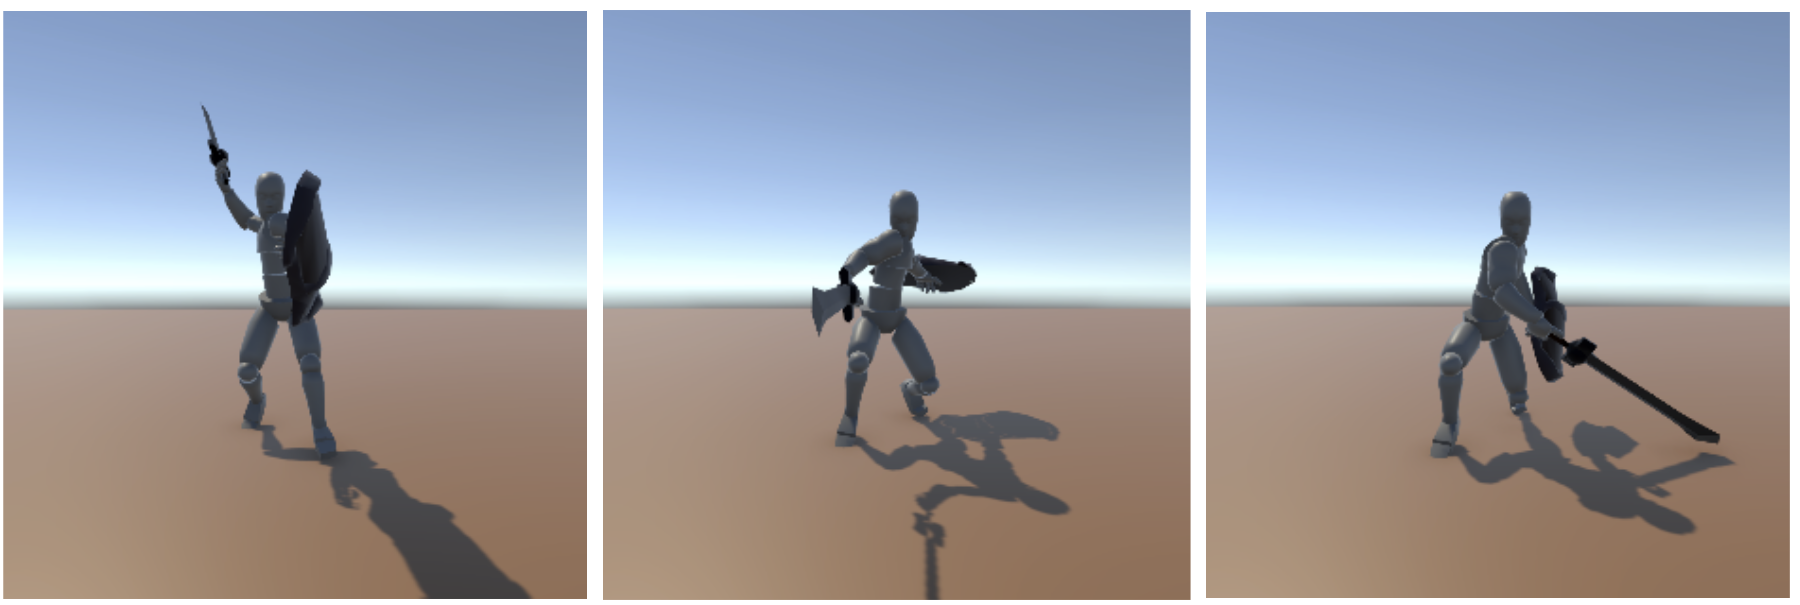
\includegraphics[width=13cm]{FrameImage/Attack1.png}
    \caption{Attack1,WeakAttack1}
    \label{}
  \end{center}
\end{figure}

\begin{figure}[htbp]
  \begin{center}
    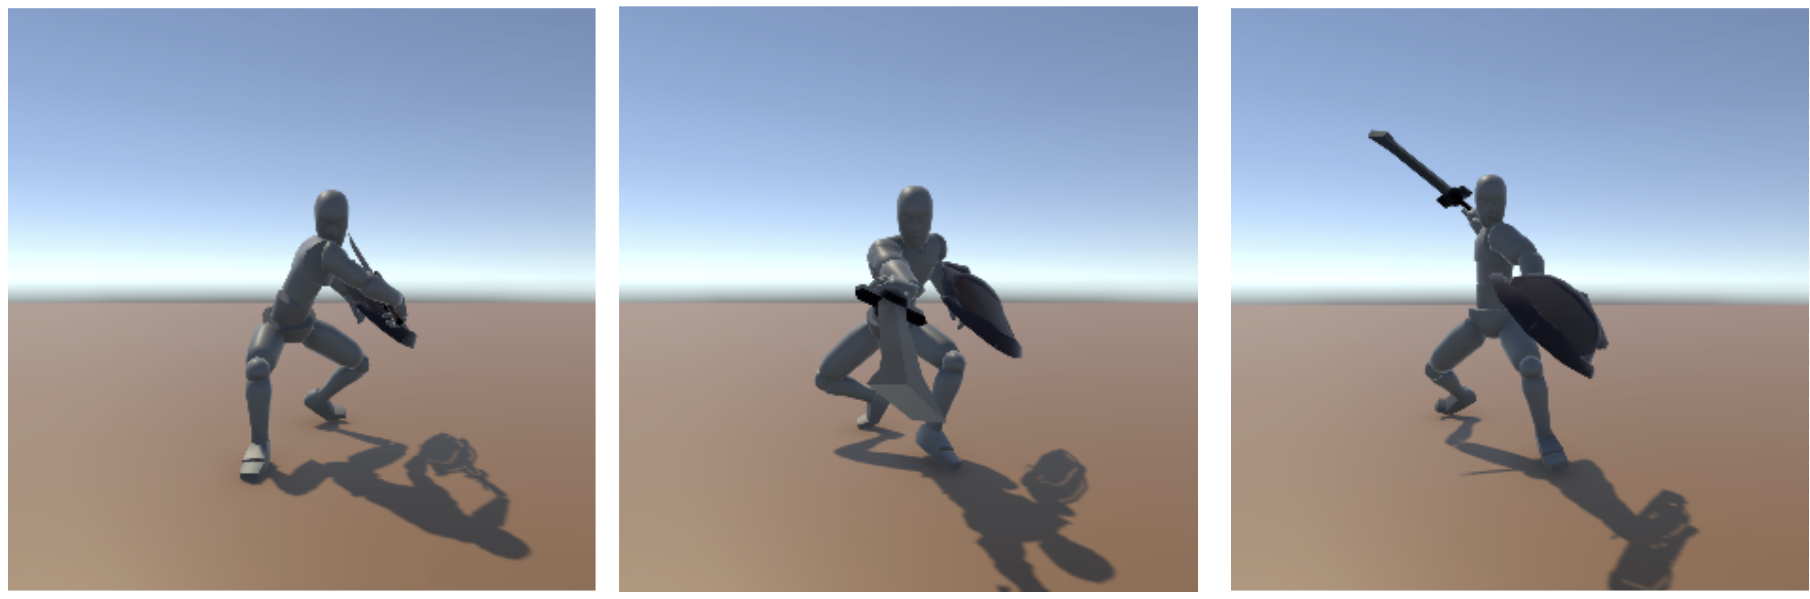
\includegraphics[width=13cm]{FrameImage/Attack2_rolling.png}
    \caption{Attack2,RollingAttack,WeakAttack2}
    \label{}
  \end{center}
\end{figure}

\begin{figure}[htbp]
  \begin{center}
    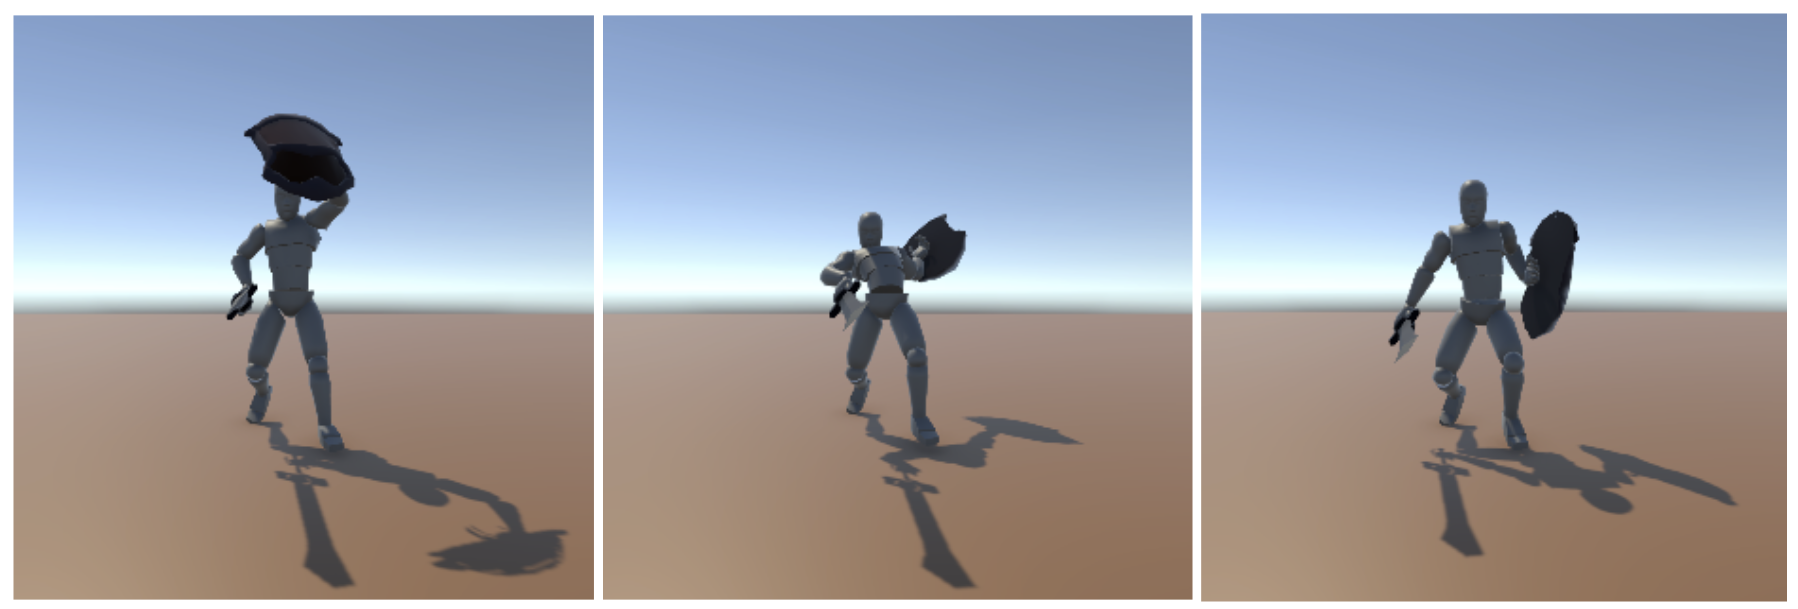
\includegraphics[width=13cm]{FrameImage/GuardBreak.png}
    \caption{GuardBreak}
    \label{}
  \end{center}
\end{figure}

\begin{figure}[h]
  \begin{center}
    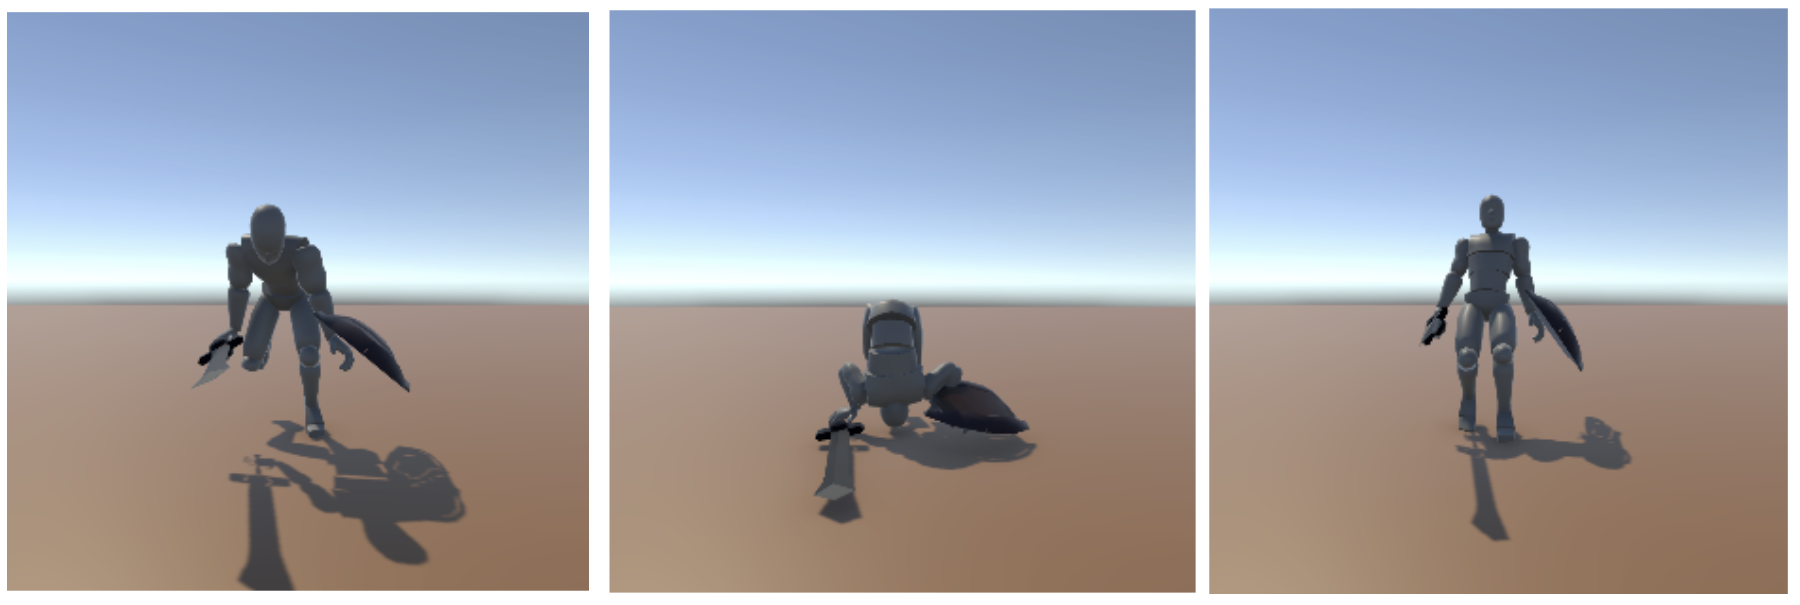
\includegraphics[width=13cm]{FrameImage/Rolling.png}
    \caption{Rolling}
    \label{}
  \end{center}
\end{figure}

\begin{figure}[h]
  \begin{center}
    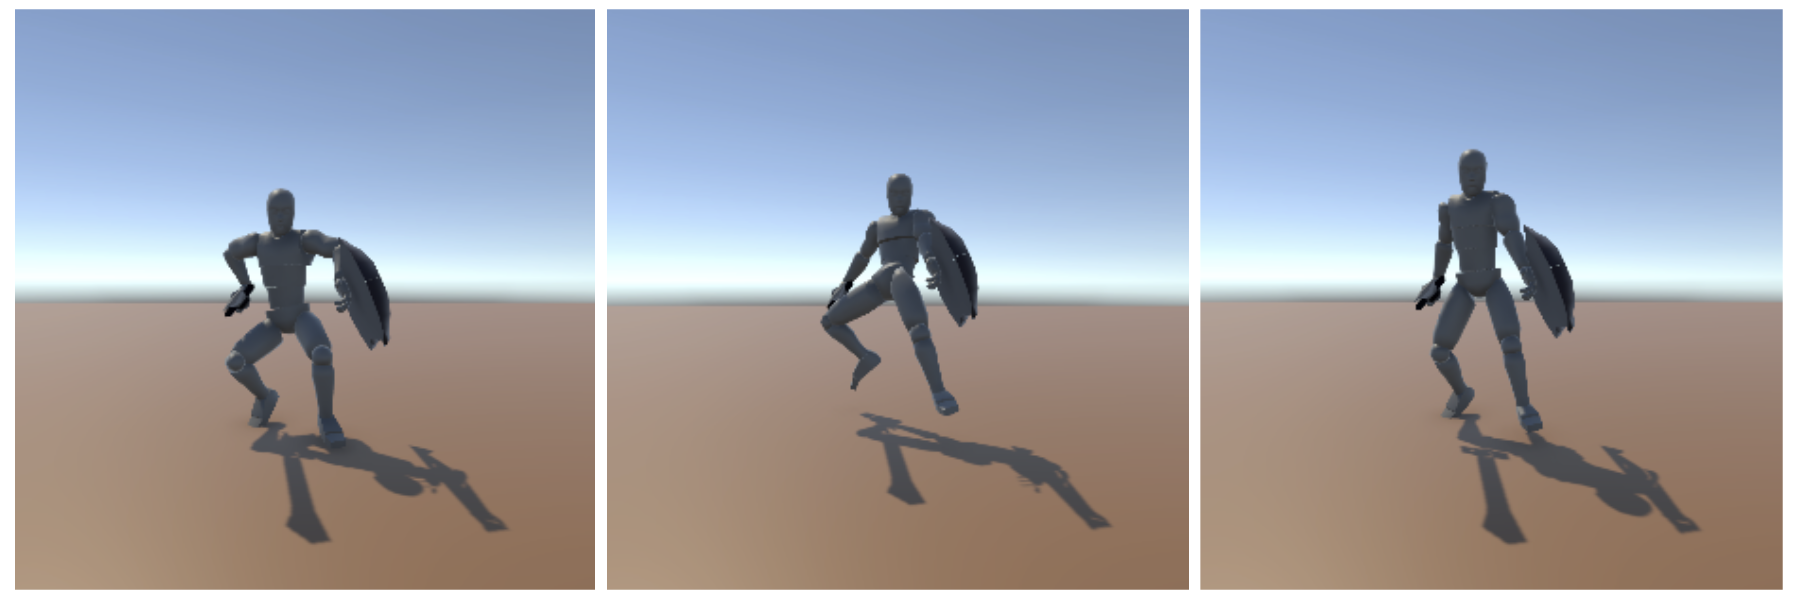
\includegraphics[width=13cm]{FrameImage/BackStep.png}
    \caption{BackStep}
    \label{}
  \end{center}
\end{figure}

\begin{figure}[h]
  \begin{center}
    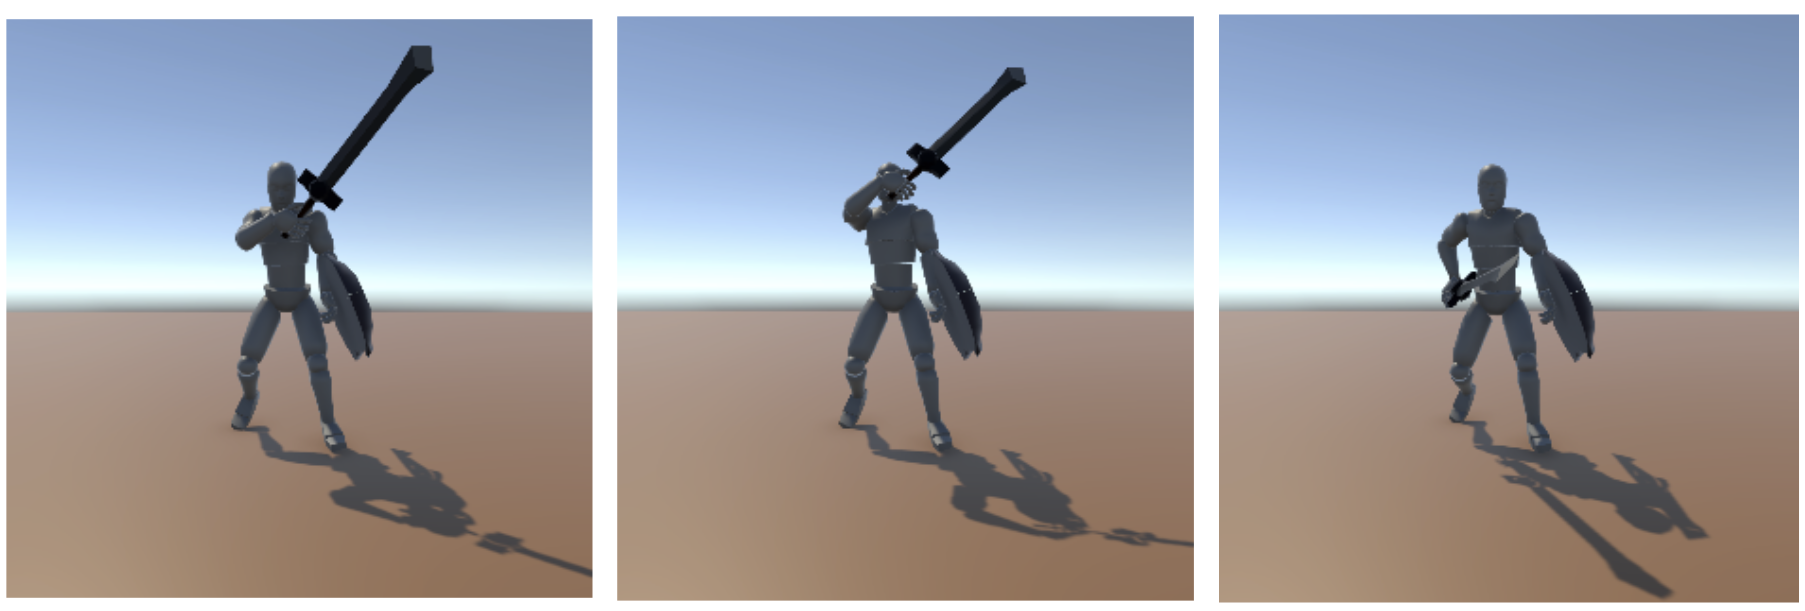
\includegraphics[width=13cm]{FrameImage/Heal.png}
    \caption{Heal}
    \label{}
  \end{center}
\end{figure}

\begin{figure}[h]
  \begin{center}
    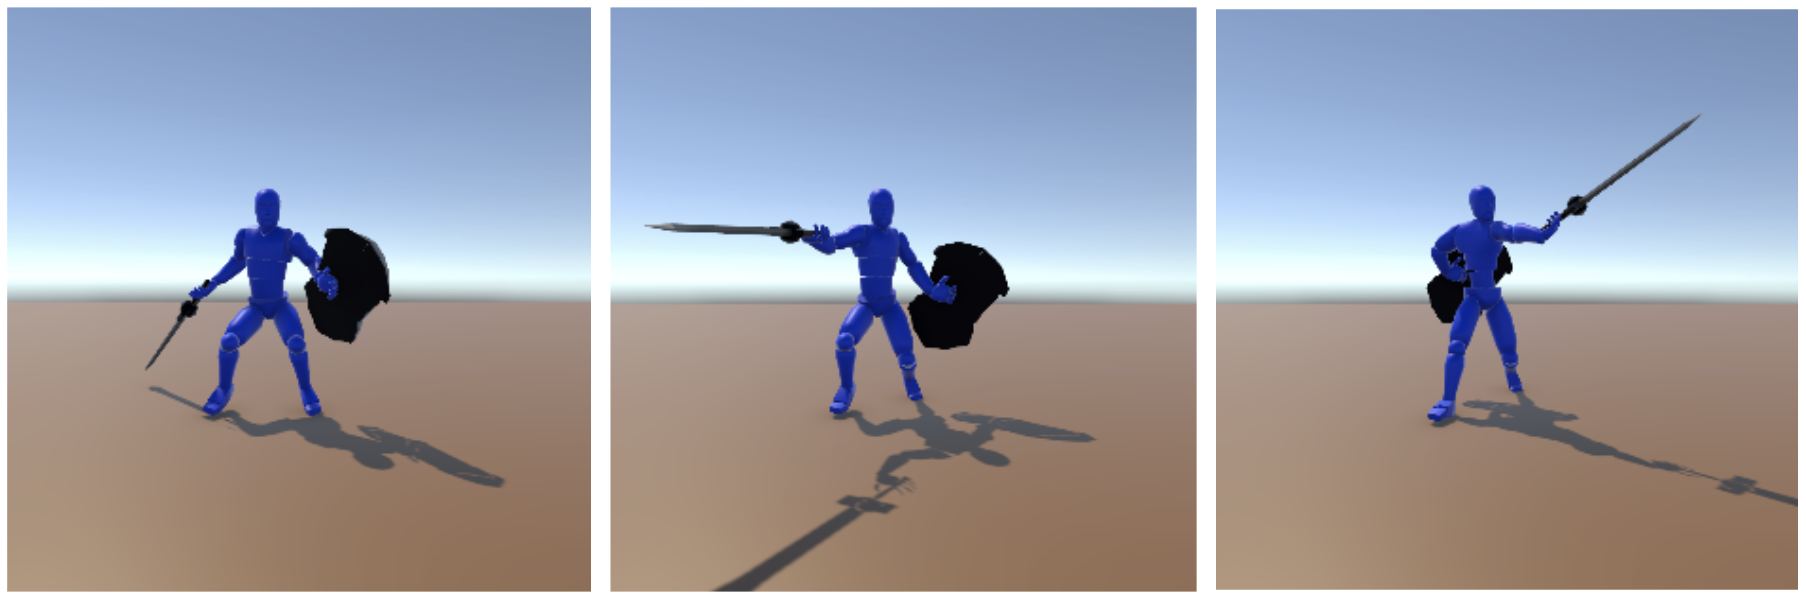
\includegraphics[width=13cm]{FrameImage/Attack3.png}
    \caption{WeakAttack3}
    \label{}
  \end{center}
\end{figure}
\begin{figure}[h]
  \begin{center}
    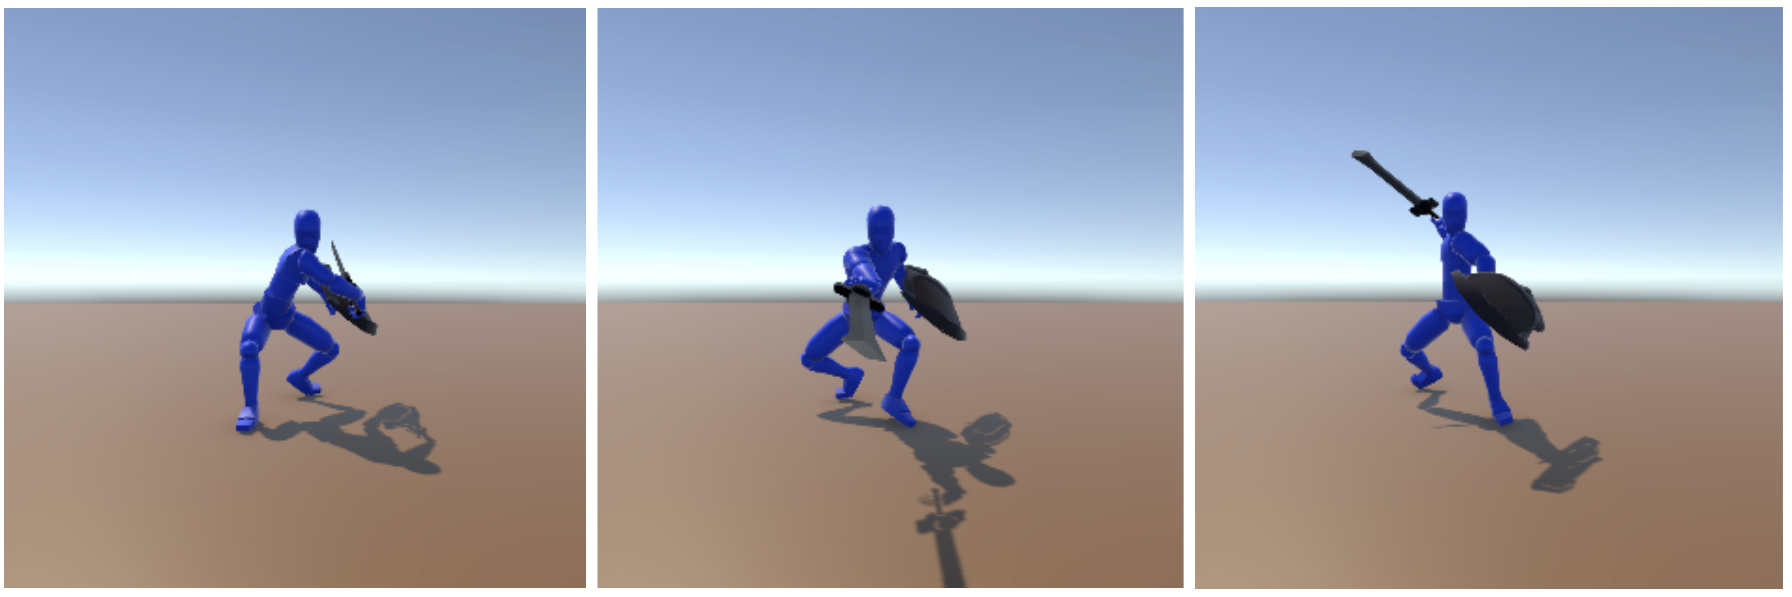
\includegraphics[width=13cm]{FrameImage/Attack4.png}
    \caption{WeakAttack4}
    \label{}
  \end{center}
\end{figure}
\begin{figure}[h]
  \begin{center}
    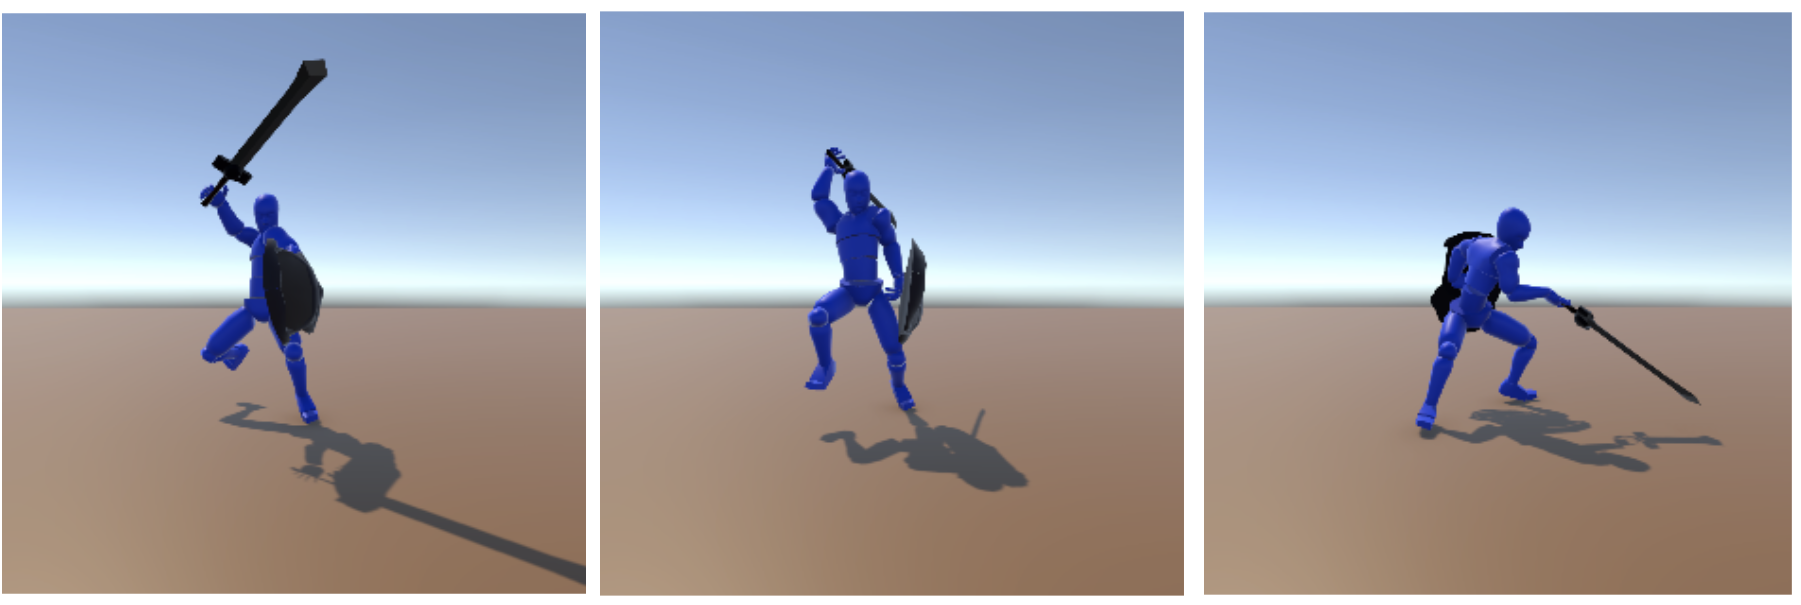
\includegraphics[width=13cm]{FrameImage/Attack5.png}
    \caption{WeakAttack5}
    \label{}
  \end{center}
\end{figure}
\begin{figure}[h]
  \begin{center}
    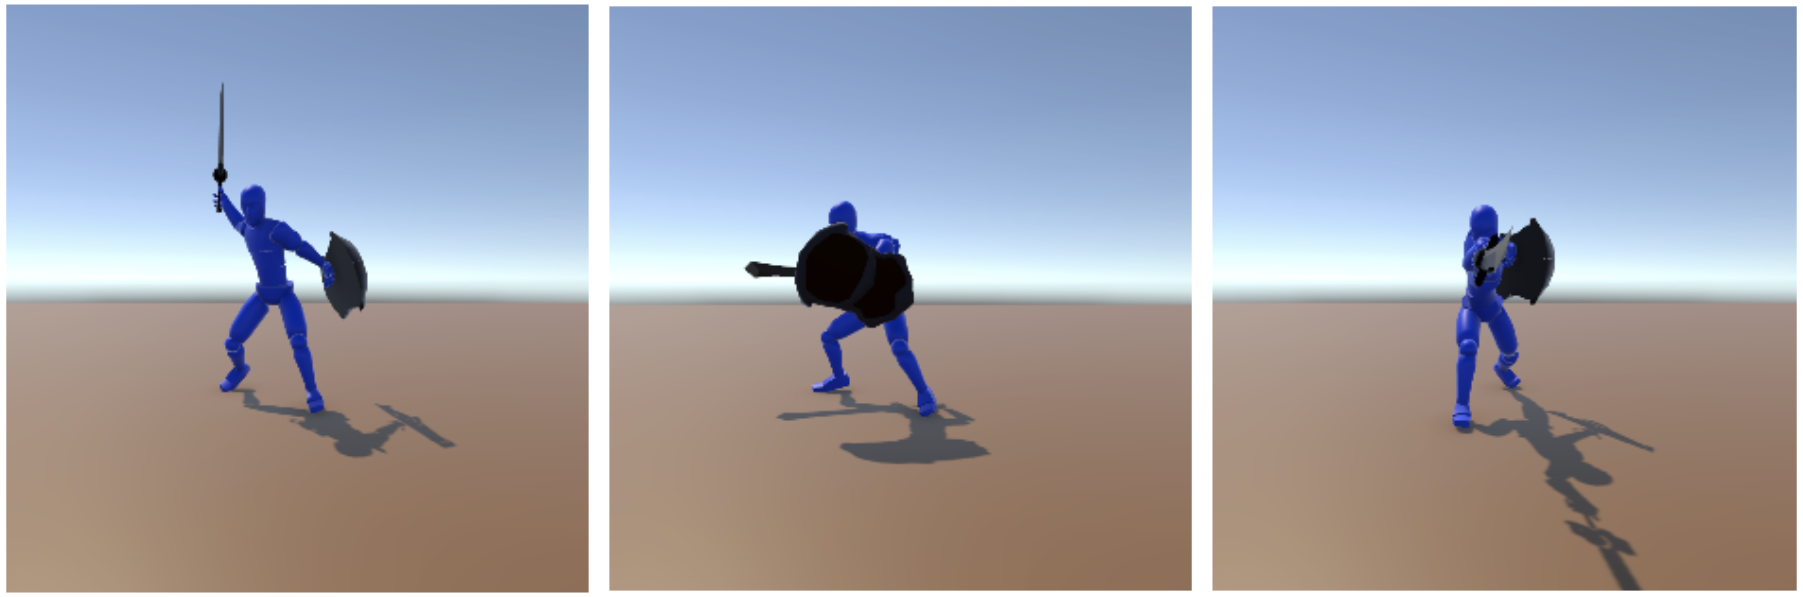
\includegraphics[width=13cm]{FrameImage/SuddenApproach.png}
    \caption{StrongAttack1,RushAttack}
    \label{}
  \end{center}
\end{figure}
\begin{figure}[h]
  \begin{center}
    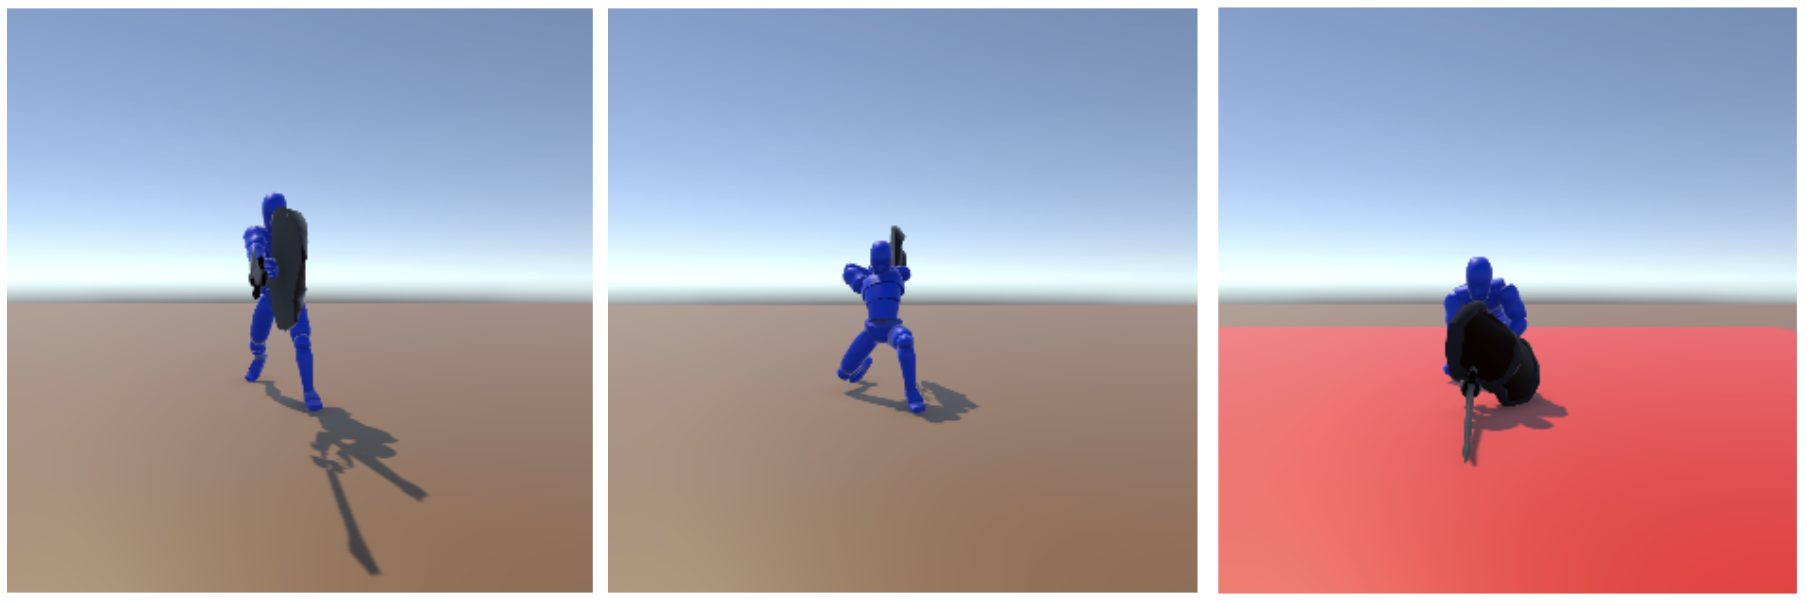
\includegraphics[width=13cm]{FrameImage/BossAttack1.png}
    \caption{StrongAttack2}
    \label{}
  \end{center}
\end{figure}
\begin{figure}[h]
  \begin{center}
    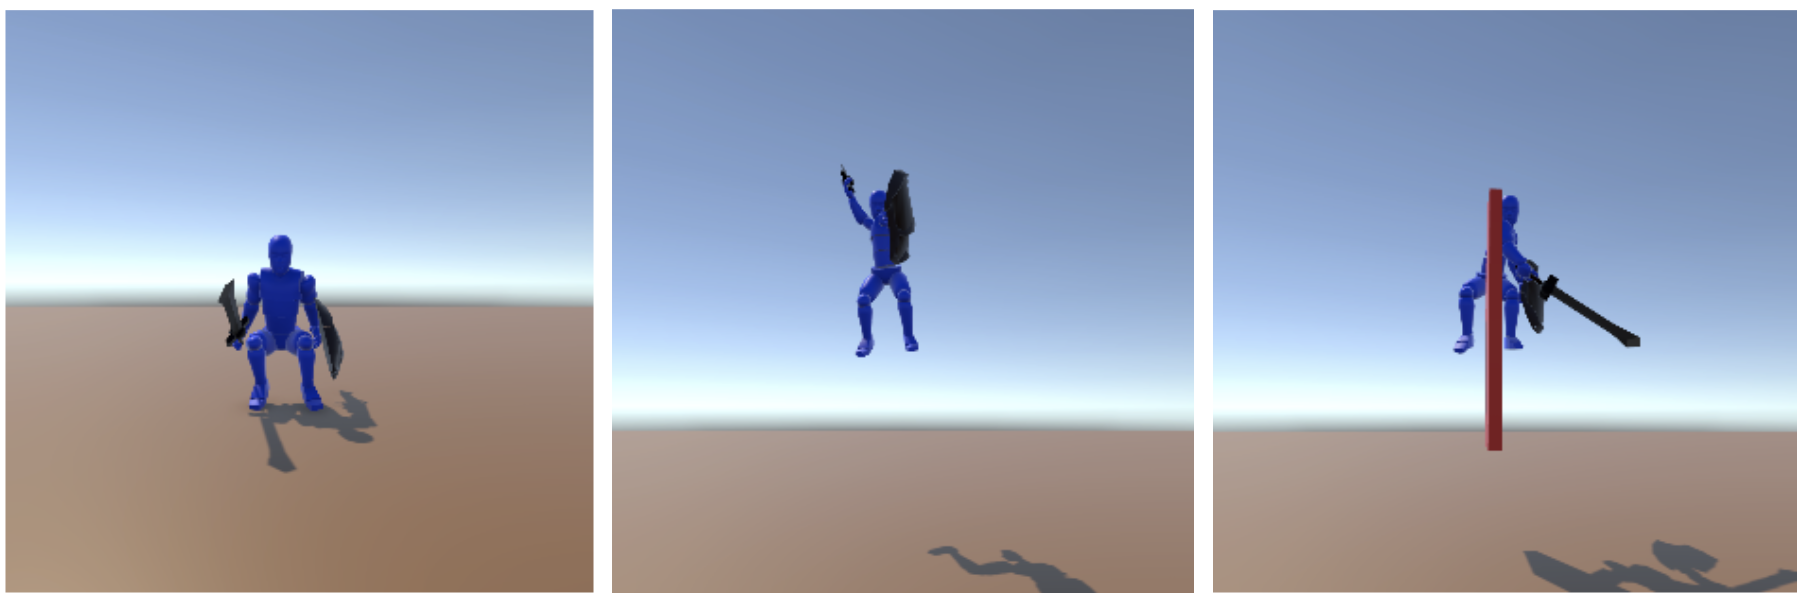
\includegraphics[width=13cm]{FrameImage/ShootWeapon.png}
    \caption{ShootAttack}
    \label{}
  \end{center}
\end{figure}




\newpage

\addcontentsline{toc}{chapter}{\bibname}
% \chapter*{\bibname}
% \thispagestyle{plain}
% \lhead{\leftmark}
% \rhead{\thepage}
% \renewcommand{\headrulewidth}{1pt}
\begin{thebibliography}{99}
\bibitem{morita}   森田 隆弘,DQNと生物学的制約を用いた
人間らしい振る舞いのゲームAI,
第124回人工知能基本問題研究会(SIG-FPAI)

\bibitem{tutii}  土居 海里,竹内 聖悟,
生物学的制約による人間らしい対戦テトリスAIの研究,
ゲームプログラミングワークショップ2023論文集,pp. 42-47,
2023.

\bibitem{fujiyama} 藤山 仁聖,清 雄一,田原 康之,大須賀 昭彦,
マルチプレイヤRPGにおいて人間らしいプレイスタイルをとるゲームAIの提案,
第16回データ工学と情報マネジメントに関するフォーラム,
2024.

\bibitem{darksouls} DARKSOULS https://www.darksouls.jp
\bibitem{niou} 仁王 https://www.gamecity.ne.jp/nioh/

\bibitem{FuJi_en} N. FUjii,Y. Sato,H. Wakama,K. Kazai and H. Katayose,
Proc. ACE, LNCS, vol. 8253, pp. 61-76,
Evaluating Human-like Behaviors of Video-Game Agents Autonomously Acquired with Biological Constraints,
2013.

\bibitem{dif-action} 荒木 海斗,三上 浩司,兼松 祥央,松吉 俊,
高難易度アクションゲームにおけるプレイヤー
に気づかれにくい難易度調整手法,
エンタテインメントコンピューティングシンポジウム(EC2023),
2023.

%ここから3章
\bibitem{unity} Unity https://unity.com
\bibitem{AnimRigging} Animation Rigging\\
https://docs.unity3d.com/ja/Packages/com.unity.animation.rigging@1.2

\bibitem{stress} 長谷川 弓子,矢野 円郁,小山 哲,猪俣 公宏,
プレッシャー下のゴルフパッティングパフォーマンス:
不安の強度とパッティング距離の影響,
スポーツ心理学研究,2011年38巻p.85-98.
%https://www.jstage.jst.go.jp/article/jjspopsy/38/2/38_2011-084/_article/-char/ja

\bibitem{hoyuu}大橋賢裕,保有効果を測るアンケート実験について,
経済集志,第90巻第1号,2020.
%https://drive.google.com/file/d/1yGWSp4jY-YkjWIKPpfEa-4f2VOMvZexX/view
\bibitem{fam_kouryaku}ファミ通,「エルデンリング」攻略/初心者向けバトル解説.
基本システムやテクニックを学んで,強敵たちに立ち向かおう!2022.
https://www.famitsu.com/news/202202/25252510.html

\end{thebibliography}

\newpage

\addcontentsline{toc}{chapter}{研究業績}
\chapter*{研究業績}
\thispagestyle{plain}
\lhead{\leftmark}
\rhead{\thepage}
\renewcommand{\headrulewidth}{1pt}
 \section*{研究会}
 長内 勇輝, 清 雄一, 田原 康之: 
 高難易度アクションゲームにおける人間らしいAI,  
 DEIM2025 第17回データ工学と情報マネジメントに関するフォーラム,
2025で発表予定

\newpage






\end{document}
